% Attention based Encoder-Decoder architectures for NMT proposed in \cite{bahdanau2014neural} and \cite{luong2015effective} are discussed. In the next section, I discuss about unsupervised morphological induction technique from \cite{soricut2015unsupervised}.

%In this chapter, we describe in detail about the problem of translation morphologically rich languages and the proposed vocabulary expansion technique as a solution to the problem. First, we present why it is difficult to translate morphologically rich language. Then, the proposed approach and its components are presented. Finally, the architecture and implementation details of the different modules is presented. 

%This chapter discusses about the objective of this project and the modules that were implemented. First the objective of the project is presented. Then, we will look into various components of the project; their architecture; implementation details. In the last section, I talk about the vocabulary expansion method that I am studying in this project.

%the vector representation for all words can be generated using external monolingual corpus. Using this fixed word vectors as input, the NMT systems are trained under limited vocabulary.



In this Chapter, we present our proposed approach for improving the quality of machine translation for morphologically rich languages. In Section \ref{sec:problem}, we present the challenges in translating a language with rich morphology. In Section \ref{sec:propose}, we describe in detail the proposed vocabulary expansion technique as a solution to the problem. All the components implemented for this study and their architectures are presented in Section \ref{sec:components}. Finally, in Section \ref{sec:implementation}, the implementation details of all the modules are discussed.


\section{Problem}
\label{sec:problem}
NMT systems have been very successful in achieving state-of-the-art performance for many language pairs such as English-French and English-German. However, these systems are not capable of translating rare and unknown words \citep{luong2015addressing}. All NMT systems have a fixed vocabulary of 30k-80k most frequently occurring words. So, words that do not occur or occur rarely in the training data will not get good vector representations. This results in poor translation performance on sentences with rare and unknown words (a.k.a OOV words) \citep{sutskever2014sequence,bahdanau2014neural}. 


This problem with translating OOV words is more pronounced in morphologically rich languages like Turkish, German, Tamil etc. There are two factors that primarily contribute to this:
\begin{itemize}
	\item In morphologically rich languages, due to inflections, there are many possible \textit{word forms} per lexeme as shown in Table \ref{turkish}. For example, even in a morphologically impoverished language like English, we have \textit{run, running, ran, runs} which are all the forms of the same lexeme \textit{run}. So, the vocabulary size in these languages is very high resulting in \textbf{more OOV words}. 
	
	\item NMT requires a large amount of training data for higher performance. Many of these languages have a much  \textbf{less data} available for training a translation system. For example, there are only 300k sentence pairs available for Turkish-English and approximately 200k sentence pairs available for Tamil-English. 
\end{itemize}

To overcome these problems, we need a system that can handle OOV words effectively by understanding the morphology of the words. This system should be capable of mapping the OOV words to an in-vocabulary word using morphological transformations. So, to address this problem, we need to answer the following questions:

\begin{enumerate}
	\item How do we get vector representations for OOV words, that captures the linguistic properties of a word?
	\item Can we improve the performance of NMT systems using vector representations that exhibit linguistic regularities?
\end{enumerate}

%Two factor co where the available data is sparse compared to vocabulary size in these languages. 

%This required handling rare and unknown words in translation systems, particularly under low resource settings. 

\section{Proposed Vocabulary Expansion Technique}
\label{sec:propose}
The main objective of this project is to improve the quality of machine translation for morphologically rich languages by incorporating morphological information. In particular, we focus on improving the translation quality under low-resource settings - when only a smaller amount of data is available for training. To address this problem in NMT systems, we propose and study a simple source vocabulary expansion technique that can translate any source word. 

Word embedding models proposed in \cite{mikolov2013distributed,pennington2014glove}  have been shown to exhibit linguistic regularities in the form of semantics  and morphology as shown in eq 4.1 and eq 4.3 \citep{soricut2015unsupervised}. 

\begin{align}
\vec{\textit{man}} - \vec{\textit{woman}} + \vec{\textit{king}} &  \approx \vec{\textit{queen}} \\
\vec{\textit{stop}} + (\vec{\textit{walking}} - \vec{\textit{walk}}) & \approx \vec{\textit{stopping}} \\
\vec{\textit{stop}} + \vec{(\textit{suffix:ing})} & \approx \vec{\textit{stopping}} 
\end{align}


Inspired by this observation, we hypothesize that fixed word embeddings can be used to expand the source side vocabulary in any NMT system. Instead of letting the NMT system learn word representation, we use a \textit{fixed} pre-trained word representation during training. During training, the NMT system learns the mapping from source language word embeddings to target language word embeddings. 

By fix the word embedding, we achieve the following benefits:
\begin{itemize}
	\item We retain the linguistic regularities present in word representations and feed them to a translation system.
	\item We reduce the number of parameters to tune for NMT systems resulting in faster training.
\end{itemize}


During testing, for any OOV source language word, we generate a word representation which maintains the linguistic regularities. Consider this example: We have a vector $\vec{(suffix:ed)}$ that can transform all the present tense words to their corresponding past tense word in the vector space. If we encounter an OOV word like \textit{$\vec{enthralled}$}, we can use the vector for the in-vocabulary word \textit{$\vec{enthrall}$} and $\vec{(suffix:ed)}$ to generate a meaningful vector representation. This vector can now be fed into the NMT system instead of mapping it to \textit{unk} word. There have been many approaches proposed that make use of pre-trained word embeddings. But, to the best of our knowledge, vocabulary expansion based on fixed word embedding have not been studied.

%this is the first time a vocabulary expansion technique based on fixed word embeddings is proposed.

%To get good vector representation for OOV words, I have compared different approaches for it on a standard data-set for their performance. The best performing models is then taken and used as an input 


To generate these morphological transformations, we experiment with two models: 
\begin{itemize}
	\item Language agnostic, unsupervised morphological transformation approach from \cite{soricut2015unsupervised}
	\item Word representation using subword information from \cite{bojanowski2016enriching}
\end{itemize}

From our experiments, discussed in next chapter, we find that \citeauthor{bojanowski2016enriching}'s approach generates a more accurate vector OOV word. We use this model in our final NMT system. To study the effectiveness of the proposed approach, we implement this technique on a baseline model and report the performance gains. For baseline NMT systems, we implement the global-attention based encoder-decoder RNN model from \cite{luong2015effective}. 

%They use a soft attention model that determines which words to focus in source language while generating target language words.

%For morphological analyser, I will extend the work of \cite{soricut2015unsupervised} where they proposed an language-agnostic, unsupervised method for inducing morphological transformation between words.


\section{Project Components}
\label{sec:components}
In this section, we discuss the baseline NMT systems and the morphological analyzer implemented for this project. The architecture of these two systems is explained in detail below.
%For this project, we implemented and used the following system:
%\begin{itemize}
%	\item An global attention based NMT system \cite{luong2015effective}.
%	\item Morphological analyzer proposed in \cite{soricut2015unsupervised} to handle rare and unknown words.
%\end{itemize}

%
%In this project, we will focus on the two problems in NMT systems. 
%\begin{enumerate}
%	\item We will study the performance of existing methods
%	in generating vector representation for OOV words based on their morphology. 
%	\item We will demonstrate the effectiveness of the proposed source side vocabulary expansion technique in NMT systems. 
%\end{enumerate}
%

%In this project, I am implementing and studying a simple vocabulary expansion technique for NMT systems, based on word morphology. 


%Although the technique was proposed for lexicon generation, the morphological rules and their vector representations learned by the technique can be used to produce vector representations for OOV words in NMT systems.




\subsection{Global Attention Based Model}
Simple encoder-decoder NMT models \citep{sutskever2014sequence,cho2014learning} do not translate long sentences very well. To overcome this problem, attention-based NMTs are used. Their networks learn word alignments between the source and target language sentence.  \cite{luong2015effective} proposed two simple but effective attention based NMT models as an alternative to the attention model from \cite{bahdanau2014neural}. 

Similar to \citeauthor{bahdanau2014neural}'s approach, their \textit{global attention} model focuses on all the source words for every target word. Their \textit{local attention} model focuses only on a small subset of the source words. For this project, we use the global attention model as the baseline.


\begin{figure}[ht]
	\centering
	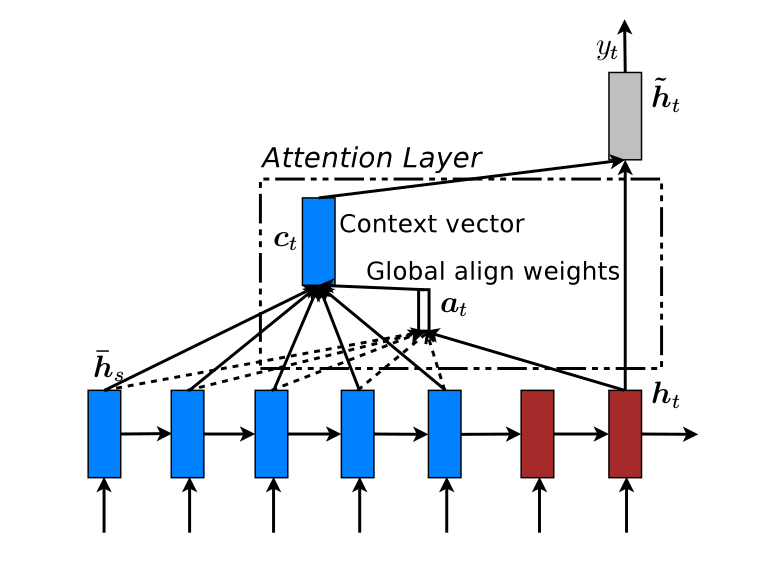
\includegraphics[scale=0.5]{images/global_attention}
	\caption{Attention based encoder. Figure taken from \cite{luong2015effective}}.
	\label{global_attention}
\end{figure}

Figure \ref{global_attention} presents a visual representation of the global attention model. The context vector $c_t$ is calculated based on alignment weights $a_t$ for every target word. To calculate attention weights, they experimented with three different scoring functions as shown in eq \ref{luong_score}. They noted that with the global attention model, a simple \textit{dot} product between encoder and decoder hidden layer vectors performs the best. We use this model with \textit{dot product} as the scoring function.

\begin{align}
\label{luong_score}
score(\overrightarrow{h_j}, s_i) =
\begin{cases}
\overrightarrow{h_j} ^\top s_i & dot \\
\overrightarrow{h_j} ^\top \textbf{W}_a s_i & general \\
v_a ^\top \textbf{W}_a [ \overrightarrow{h_j}, s_i ] & concat
\end{cases}
\end{align}


%\cite{bahdanau2014neural} proposed an attention based encoder-decoder architecture which is capable of learning word alignment between source and target sentences. This allowed for the encoder to produce better sentence representation for longer sentence which in turn improved the translation quality. In their additive approach, a single feed forward neural networks that can learn to assign different weights to the hidden layer vectors was used. These weighted sum of the hidden layer vectors $h_{1:n}$ called context vectors $c_i$ is calculated each time decoder generates a new word as shown in figure \ref{attention}.
%
%
%\begin{align*}
%c_i &= \sum_{j=1}^{n} \alpha_{ij} h_j \\
%\alpha_{ij} &= \frac{\hat{a}_{ij}}{\sum_j \hat{a}_{ij}}\\
%\hat{a}_{ij} &= att(s_i, h_j)
%\end{align*}
%
%where $att(s_i, h_j)$ is an attention function that calculates the weights for each encoder hidden state $h_{1:n}$ for a given decoder state $s_i$. %\cite{bahdanau2014neural} also used bi-directional RNN which reads the sentence from both directions. The state vector from both direction right to left  $\overleftarrow{h_i}$ and left to right $\overrightarrow{h_i}$ is concatenated for each word. The attention mechanism is applied over this concatenated hidden state vector $h_i = [\overleftarrow{h_i};\overrightarrow{h_i}]$. The whole network is trained with negative log-likelihood as objective function using stochastic gradient descent.

\subsection{Unsupervised Morphological Analyzer}

\cite{soricut2015unsupervised} proposed a language-agnostic, heuristic method to capture morphological transformations by exploiting regularities present in word embeddings \citep{mikolov2013distributed}. Their method automatically deduces morphological rules and transformations from word vectors. These morphological transformations can be represented as vectors in the same embedding space. During testing, OOV words can be mapped into the same vector space using the learned morphological transformations. In this algorithm, the morphological rules are learned as follows.


\begin{figure}[ht]
	\centering
	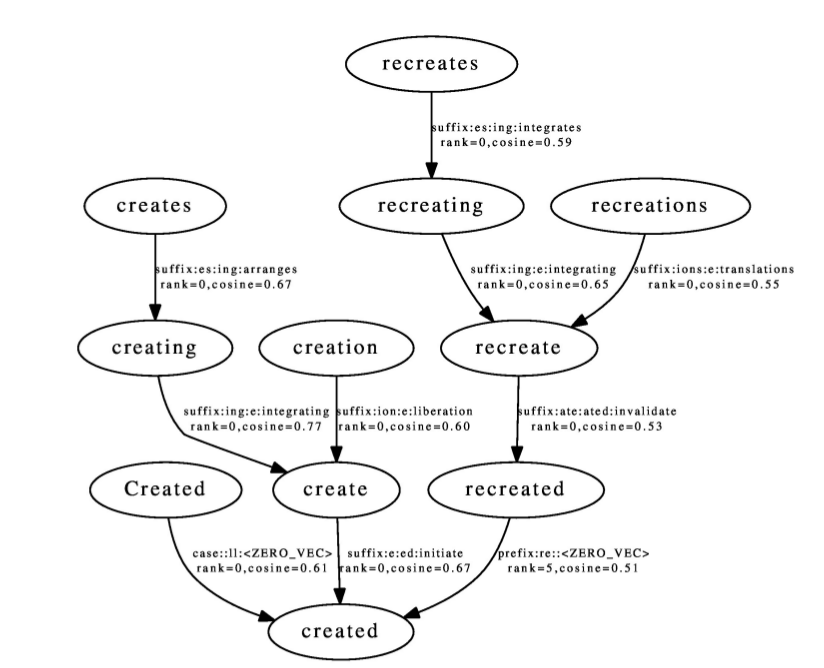
\includegraphics[scale=0.5]{images/morph_graph}
	\caption{A part of normalized, directed graph with morphological mapping. Figure taken from  \cite{soricut2015unsupervised}}.
	\label{graph_morph}
\end{figure}

\begin{enumerate}
	\item Extract candidate morphological rules like \textit{('suffix', 'ies', 'y')} (replace suffix \textit{ies} with \textit{y} from the word \textit{treaties} to get \textit{treaty}) from every possible word pairs in vocabulary V. 
	\item Then, evaluate the quality of rules in the pre-trained embedding space by calculating the hit-rate for other word pairs.
	\item Generate morphological transformation from the above candidate rules and build a cyclic multi-graph, where words form the nodes and edges form the morphological transformations. The edges between the words are weighted using cosine distance between their vectors and their ranks $(rank, cosine)$.
	\item From the above graph, build a normalized acyclic graph with 1-1 morphological mapping between words. This graph is normalized by mapping low-frequency words to high-frequency words as shown in Figure \ref{graph_morph}. In this graph, all the low-frequency words in the dataset \textit{(recreates, recreations, creates)} are mapped to higher frequency words \textit{(create, created)}.
	\item Use the final graph and the learned morphological transformations to map the rare/out of vocabulary words in the same vector space.
\end{enumerate}

%\subsubsection{Candidate Rule Extraction}
%For every word pair $(w_1 , w_2 )$ in vocabulary $V$, all possible prefix and suffix substitutions from $w_1$ to $w_2$ of predefined length 6 are extracted. For each rule $r$, its support set $S_r$ - set of all word pair that obey rule $r$, is extracted.
%
%\[ S_r = \{(w_1 , w_2 ) \in V^2 |w_1 \xrightarrow{r} w_2 \} \]
%
%
%\subsubsection{Evaluate candidate rules}
%The hit rate for each rule is computed using cosine rank. For every word-pair combination in $S_r \times S_r$, we can calculate the percent of the time similairity rank is higher than the threshold $t_{rank}$. For word pair $((walking, walk),(talking, talk))$, the rank of $(walking, walk + \uparrow d_{talk\_\_})$ was computed.  It can be seen that meaning preserving rules like $suffix:ed:ing$ receive high hit rate while non meaning preserving rule receive low hit rate.
%
%
%
%\subsubsection{Generate Morphological Transformation}
%
%
%For each rule $r$, the best direction vector $\uparrow{d_w}$ is computed greedily. The direction vector $\uparrow{d_w}$ which explains most of the word pair in support is selected recursively for all unexplained word pairs. By doing this, we will have the morphological transformations for each rule. These morphological transformations are subject to further evaluation using cosine similarity and cosine similarity rank. The cosine similarity threshold was set to $t_{cosine}$ = 0.5 and cosine rank threshold was set to $t_{rank}$ = 30. If these thresholds are not met, the rules are removed.
%
%
%The morphological transformations also have a graph based interpretations. A labelled, weighted,	, directed multi-graph $G^V_{Morph}$ is created from the transformations where nodes are the words in vocabulary and edges are the morphological transformation with $(rank, cosine)$ as the weights. From all the candidate morphological transformations 1-1 mappings are selected based on the the following conditions.
%
%\begin{itemize}
%	\item Edges are considered only if they start from higher count word and end at lower count word.
%	\item If multiple edges exist, the ones with minimal rank $rank$ is selected.
%	\item If multiple edges still exist, the one with maximum $cosine$ is selected.
%\end{itemize}
%
%This normalizes the graph to weighted directed graph $D^V_{Morph}$ where low occurring words are mapped to high occurring words using a direction vector.
%
%
%\subsubsection{Mapping Rare and Unknown Words}
%The word vectors for out of vocabulary words, and low frequency words can generated by mapping them to nodes in $D^V_{Morph}$ using the morphological rules. $V_c$ is the set of all low frequency words and OOV words.
%
%\[ V_c=\{w \in V|C\leq count(w)\} \]
%
%All the morphological rule $r\in R$ are applied on words $w\in V_c$ and if any of them results in a word $w'\in D^V_{Morph}$ then that word is mapped into the graph using the direction vector for rule $r$. This allows us to get meaning full representation for Rare and Unknown words at testing time.


Using this approach, if the word \textit{unassertiveness} occurs in the source sentence and is not found the vocabulary of the word embedding model, we would still be able to get a meaningful vector representation for the word. Traditionally, any word not in the vocabulary is mapped to the token \textit{unk}. Using this approach, we can learn vector representation for morphological transformations like \textit{(prefix,un,$\epsilon$)} and \textit{(suffix,$\epsilon$,ness)}. These morphological rules and their vector representation can then be used to map the OOV word \textit{unassertiveness} to  \textit{assertive} and get a good vector representation. 



\section{Implementation Details}
\label{sec:implementation}
In this section, we will present the implementation details of \textit{attention based NMT} and \textit{morphological analyzer} for this project.

The baseline NMT system was implemented from scratch in \textit{pytorch}, a deep learning framework. Later, we switched to \textit{OpenNMT-py}\footnote{https://github.com/OpenNMT/OpenNMT-py} for the fine-tuned performance gains it offers. OpenNMT-py is a collaborative research-friendly framework focusing specifically on machine translation. 

We implemented the morphological analyzer purely in Python. We used \textit{gensim\footnote{https://github.com/RaRe-Technologies/gensim}} to calculate word similarities and their rank in the vector space. For building and storing graphs, we used \textit{networkx\footnote{https://networkx.github.io}} graph library. Finding the nearest neighbour in 300 dimension vector space, with 3M candidates is expensive. Since we do this calculation many time for each word, it can takes days to run on a standard computer. To speed up computation, we used k-d tree based Approximate Nearest Neighbour (ANN) algorithms from \textit{annoy}\footnote{https://github.com/spotify/annoy} library under low precision settings.

%For finding nearest neighbour in vector space, we used annoy\footnote{https://github.com/spotify/annoy} library. 
%Major chunk of the time was spent on optimizing the run-time and memory usage of the program.